\documentclass[main.tex]{subfiles}

\begin{document}
 
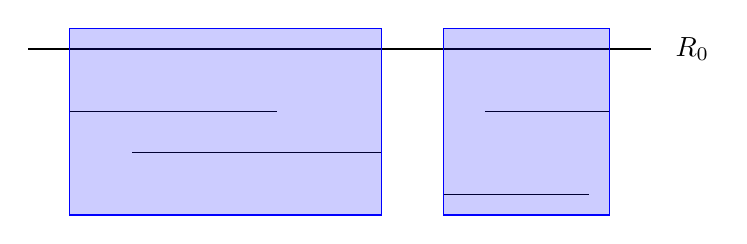
\begin{tikzpicture}[x=0.75pt,y=0.75pt,yscale=-1,xscale=1]

\draw (30, 0) -- (330, 0);
\draw (50, 30) -- (150, 30);
\draw (250,30) -- (310,30);
\draw (80, 50) -- (200, 50);
\draw (230, 70) -- (300, 70);

\draw [blue, fill=blue, fill opacity=0.2] (50, -10) -- (50, 80) -- (200, 80) -- (200, -10) -- cycle;
\draw [blue, fill=blue, fill opacity=0.2] (230, -10) -- (230, 80) -- (310, 80) -- (310, -10) -- cycle;

\draw (350, 0) node {\texttt{$R_0$}};

\end{tikzpicture}

\end{document}